\documentclass{article}
\usepackage{graphicx} % Required for inserting images
\usepackage{amsmath} 
\usepackage{listings}
\usepackage{xcolor}
\usepackage{float}

\lstset{ 
  language=Python,                % El lenguaje del código
  basicstyle=\ttfamily\footnotesize, % Estilo básico del texto
  keywordstyle=\color{blue},    % Color para palabras clave
  commentstyle=\color{green},   % Color para comentarios
  stringstyle=\color{red},      % Color para strings
  numbers=left,                 % Números de línea a la izquierda
  numberstyle=\tiny\color{gray},% Estilo de los números de línea
  stepnumber=1,                 % Números de línea en cada línea
  numbersep=5pt,                % Separación entre números de línea y código
  backgroundcolor=\color{white},% Color de fondo
  showspaces=false,             % No mostrar espacios
  showstringspaces=false,       % No mostrar espacios en strings
  showtabs=false,               % No mostrar tabs
  frame=single,                 % Cuadro alrededor del código
  tabsize=2,                    % Tamaño de tabulación
  captionpos=b,                 % Título debajo del código
  breaklines=true,              % Cortar líneas largas
  breakatwhitespace=false,      % Cortar solo en espacios
  escapeinside={\%*}{*)}        % Añadir LaTeX dentro del código
}

\title{Nivel 4 Introduccion a Programacion}
\author{Tomas Rodriguez - 202212868}
\date{Mayo 2022}

\begin{document}
\maketitle
\section{Tuplas}
Son estructuras de datos lineales en las cuales cada elemento tiene un indice o una posicion, es decir funcionan como las listas. Sin embargo, se sabe que las listas son mutables, es decir, se pueden agregar, eliminar y modificar sus elementos), pero las tuplas  son inmutables, es decir, sus elementos no pueden ser modificados.
\subsection{Creacion de tuplas}
Al ser parecidas a las listas estas se declaran de la misma manera solo que con una ligera diferencia, y es que en vez de usar los corchetes cuadrados que se vieron en el N3, se usan son los parentesis a continuacion:
\begin{lstlisting}[language=Python, caption= Declaracion Tupla parentesis]
numeros = (1,2,3)
\end{lstlisting}
Otra forma de crear tuplas es por medio del empaquetado, que funciona sin los parentesis:
\begin{lstlisting}[language=Python, caption= Empaquetado en tuplas]
numeros2 = 1,2,3
\end{lstlisting}
De igual forma como hay un empaquetado, las tuplas tienen la forma de desempaquetado:
\begin{lstlisting}[language=Python, caption= Desempaquedato en tuplas]
x, y, z = numeros2
\end{lstlisting}
En este caso las variables \(x,y,z\) tomaran los valores de \(1,2,3\)
\subsection{Operaciones sobre tuplas}
Al funcionar como las listas, en las tuplas se pueden usar operaciones como:
\begin{enumerate}
    \item Indexacion
    \item Slicing
    \item funcion len()
\end{enumerate}
\section{Matrices}
Son estructuras bidimensionales de que contienen datos que se organizan en filas y columnas. En python, las matrices se representan como una lista de listas:
\begin{lstlisting}[language=Python, caption= Matriz en python]
matriz = [[1,2],[3,4]]
\end{lstlisting}
Esto tendria la representacion en:
\[
matriz = 
\begin{bmatrix}
    1 & 2\\
    3 & 4    
\end{bmatrix}
\]
\subsection{Creacion de matrices}
Las matrices se pueden crear usando ciclos y tecnicas de listas:
\begin{lstlisting}[language=Python, caption= Matriz en python con ciclos]
M = []
for i in range(0,3):
    a = [0]*6
    M.append(a)
\end{lstlisting}
De esta forma se combinan las tecnicas de listas como la del operador de \(*\), los ciclos y el metodo append() de las listas para crear una matriz de \(3 \times 6\) llena de \(0\). El resultado es el siguente:
\[
M = 
\begin{bmatrix}
    0 & 0 & 0 & 0 & 0 & 0\\
    0 & 0 & 0 & 0 & 0 & 0\\
    0 & 0 & 0 & 0 & 0 & 0\
\end{bmatrix}
\]
\subsection{Operaciones sobre Matrices}
Las operaciones de matrices son las mismas que en las listas, solo que en este caso, las matrices pueden contener datos mas complejos, como por ejemplo una matriz de tuplas para representar una imagen. 
\section{Librerias}
Las librerias son extensiones de python que facilitan procesos u operaciones que en python normal, tomarian muchisimo tiempo. Algunas de las librerias mas usadas son:
\begin{itemize}
    \item NumPy: Facilita la creacion de matrices, vectores multidimensionales junto con funciones matematicas de alto nivel.
    \item SciPy: Contiene herramientas y algoritmos matematicos.
    \item Matplotlib: Generacion de visualizaciones estaticas, animadas e interactivas.
    \item SymPy: Usada para matematica simbolica.
    \item Pandas: Manipulacion y analisis de datos.
\end{itemize}
\subsection{Matplotlib}
Es una libreria para crear y manipular graficos y contiene varios modulos.
\subsubsection{Modulo Image}
Con este modulo se puede leer una imagen y convertirla en una matriz de tuplas, donde cada tupla esta dada por \((R,G,B)\).
\begin{lstlisting}[language=Python, caption= Cargar una imagen]
import matplotlib.image as mpimg
import matplotlib.pyplot as plt
def cargar_imagen(ruta:string)->list:
    imagen = mpimg.imread(ruta).toList()
    return imagen
\end{lstlisting}
De esta forma, se carga la imagen alojada en algun directorio de nuestro pc dado por la ruta, y esta es cargada y convertida en una matriz de tuplas.
\begin{lstlisting}[language=Python, caption= Visualizar una imagen]
import matplotlib.image as mpimg
import matplotlib.pyplot as plt
def visualizar_image(imagen:list)->None:
    plt.imshow(imagen)
    plt.show()
\end{lstlisting}
De esta manera se puede visualizar la imagen con el metodo imshow() que indica image show.
\subsubsection{Modulo Pyplot}
Este modulo es uno de los mas importantes, ya que no solo es que que permite la visualizacion de las imagenes o graficos por medio del metodo show(), sino que tambien, es aquel que permite crear graficos como:
\begin{itemize}
    \item Diagrama de lineas
    \item Scatter plots
    \item Diagramas de barras
    \item Diagramas de caja y bigotes o boxplot
    \item Graficos 3D
\end{itemize}
\subsection{Pandas}
Su rol mas importante esta dado que fue creado para remplazar las hojas de calculo, es decir, excel. Este nos ayuda en la limpieza, analisis y procesamiento de datos en bruto.
\subsubsection{Estructuras de datos de Pandas}
Pandas posee 3 estreucturas caracteristicas:
\begin{enumerate}
    \item: Son de 1 dimension, normamento son las columnas de una tabla
    \item El DataF Las Srame: Son de 2 dimensiones, es decir, representa filas y columnas como una matriz
    \item El Panel: Son de 3 dimensiones y no son muy usuados.
\end{enumerate}
\subsubsection{Tipos de datos en pandas}
\begin{figure}[H]
    \centering
    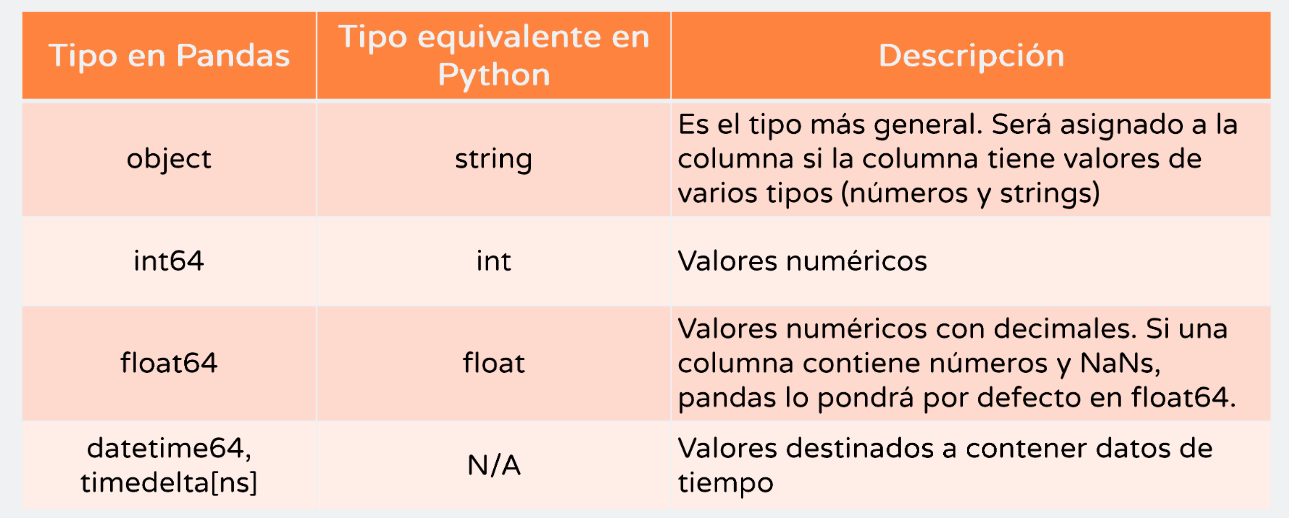
\includegraphics[width=1\linewidth]{TiposDatosPandas.png}
    \caption{Tipos de datos en Pandas}
    \label{fig:enter-label}
\end{figure}
\subsubsection{Series}
En las series, existen los indices y las posiciones o etiquetas. Estos son: 
\begin{figure}[H]
    \centering
    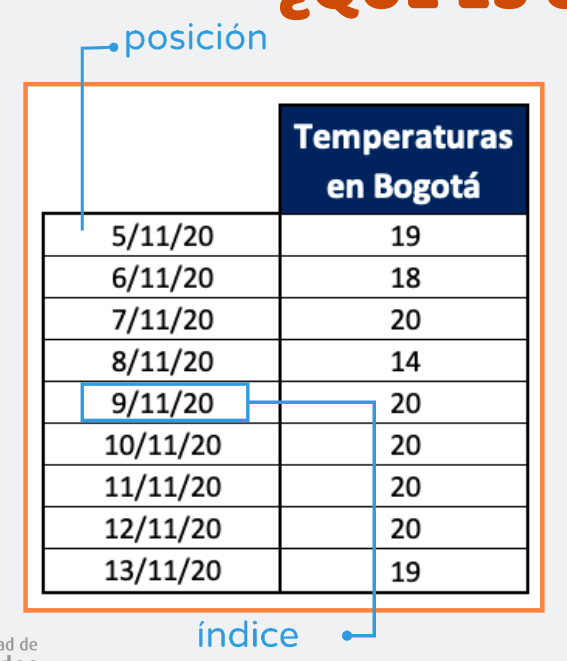
\includegraphics[width=.5\linewidth]{IndicevsPosicion.png}
    \caption{Indices vs Posicion}
    \label{fig:enter-label}
\end{figure}
La creaion de series esta dada por el siguente codigo:
\begin{lstlisting}[language=Python, caption= Creacion de una Serie]
import pandas as pd
datos = [19,18,29,14,20]
temperaturas = pd.Series(datos, name = 'Temperaturas de Bogota')
\end{lstlisting}
Y se vera una serie de la forma:
\[
\begin{bmatrix}
    1 & 19 \\
    2 & 18 \\
    3 & 29 \\
    4 & 14 \\
    5 & 20
\end{bmatrix}
\]
Donde los numeros del 1 al 5 indican los indices (primera columna) y los otros son los valores. 
\begin{lstlisting}[language=Python, caption= Creacion de una Serie con indices]
import pandas as pd
datos = [19,18,29,14,20]
fechas = ["5/11/20", "6/11/20", "7/11/20", "8/11/20", "9/11/20"]
temperaturas = pd.Series(datos, index=fechas, name = 'Temperaturas de Bogota')
\end{lstlisting}
Y se vera una serie de la forma:
\[
\begin{bmatrix}
    5/11/20 & 19 \\
    6/11/20 & 18 \\
    7/11/20 & 29 \\
    8/11/20 & 14 \\
    9/11/20 & 20
\end{bmatrix}
\]
\begin{lstlisting}[language=Python, caption= Creacion de una Serie con diccionarios]
parejas = {'5/11/20': 19, '6/11/20': 18, '7/11/20': 29,
'8/11/20': 14,  '9/11/20': 20}
temperaturas = pd.Series(parejas)
\end{lstlisting}
Y el resultado sera el mismo que el del Listing 9.\\
Ahora bien, existen ciertas operaciones en las Series que pueden ser utilies:
\begin{itemize}
    \item Reconstruir indices:
        \begin{lstlisting}[language=Python, caption= Reconstruccion de indices]
            temperaturas = temperaturas.reset_index(drop=True)
        \end{lstlisting}
        El resultado sera la serie del Listing 8.
    \item Extarer valor dado el indice: 
        \begin{lstlisting}[language=Python, caption= Extraer valor de un indice]
            valor = temperaturas.get(2)
        \end{lstlisting}
        El resultado sera el elemnto al cual pertenece el indice 2, es decir, 18.
    \item Extraer valores usando indices:
        \begin{lstlisting}[language=Python, caption= Extraer valores de indices]
            valores = temperaturas.loc[2:4]
        \end{lstlisting}
        El resultado sera:
        \[
        \begin{bmatrix}
            2 & 18\\
            3 & 29\\
            4 & 14
        \end{bmatrix}
        \]
    \item Extraer valores usando posiciones:
        \begin{lstlisting}[language=Python, caption= Extraer valores de posiciones]
            valores2 = temperaturas.iloc[2:4]
        \end{lstlisting}
        El resultado sera:
        \[
        \begin{bmatrix}
            3 & 29\\
            4 & 14
        \end{bmatrix}
        \]
    \item Extraer todos los valores en una lista:
        \begin{lstlisting}[language=Python, caption= Extraer todos los valores]
            valoresLista = temperaturas.values
        \end{lstlisting}
        El resultado sera:
        \[[
        \begin{array}{ccccc}
            19 & 18 & 29 & 14 & 20 \\
        \end{array}]
        \]
    \item Hacer una copia de la Serie:
        \begin{lstlisting}[language=Python, caption= Hacer copia de una serie]
            copia _= temperaturas.copy()
        \end{lstlisting}
        El resultado sera una copia identica a la serie pero almacenada en otro lugar en memoria
    \item Operaciones estadisticas:
        \begin{lstlisting}[language=Python, caption= Operaciones Estadisticas]
            temperaturas.max()
            temperaturas.min()
            temperaturas.mean() 
            temperaturas.std()
            temperaturas.median() 
        \end{lstlisting}
\end{itemize}
\subsubsection{DataFrames}
Los dataframes son muchos registros ordenados por columnas,m la cual cada una posee un tipo. Se pueden construir dataframes a partir de:
\begin{itemize}
    \item Lista de diccionarios
    \item Diccionario de listas
    \item Diccionario de series
    \item Archivos csv
\end{itemize}
pasra filtrar los datos y extarer las columnas de interes de un dataframe grande a uno mas pequeños se haria de la siguente manera:
\begin{lstlisting}[language=Python, caption= Copia Dataframe con columnas especificas]
columnas_valores = ['nombres de las columnas separados por comas']
valores = dataframe_original[columnas_valores].copy()
\end{lstlisting}
Aparte de estas operaciones, los dataframes tienen operaciones de analisis basico:
\begin{itemize}
    \item head(n): Deja ver las n primeras filas del dataframe
    \item tail(): Deja ver los ultimos 5 registros o filas del dataframe
    \item info(): Da informacion acerca de cada columna del dataframe
    \item describe(): Describe valores importantes del dataframe
    \item Filtrado de columnas: 
        \begin{lstlisting}[language=Python, caption= Filtrado de columnas]
            dataframe[nombre columna]
            dataframe[[nombre columna 1, nombre columna 2]]
        \end{lstlisting}
        En este filtrado, se puede hacer por una o varias columnas.
    \item unique(): Extrae un array con los valores que aparecen al menos una vez en la columna por la cula se filtra.
    \item value\_counts(): Cuenta cuantas veces aparece el valor en la columna filtrada
    \item Metodos estadisticos: mean(), mode(), std(), max(), min(), idxmax(), idxmin()
    \item Metodos matematicos: sum(), prod(), div(). Se aplican a columnas numericas como los estadisticos.
    \item ordenamiento: Se ordena el dataframe por los valores de una de las columnas:
        \begin{lstlisting}[language=Python, caption= Ordenamiento por una columna]
            ordenados = dataframe.sort_values('columna')
        \end{lstlisting}
        En estos casos ocurrira que los valores de los indices no corresponden a las posiciones.
    \item iloc[inicio:fin]: Es el mismo de la seccion de Series
    \item loc[inicio:fin]: Es el mismo de la seccion de Series
    \item Seleccion con condiciones: Es el mismo filtrado por columna, sin embargo, en este caso se usaran expresiones booleanas:
        \begin{lstlisting}[language=Python, caption= Filtrado Booleano]
            dataframe[dataframe['columna'] == algo]
        \end{lstlisting}
        En este caso se puede usar cualquier expresion booleana vista en el N2. Otra opcion es un filtrado multiple que se da de la siguente manera:
        \begin{lstlisting}[language=Python, caption= Filtrado Booleano multiple]
            dataframe[(dataframe['columna 1'] == algo) | (dataframe['columna 2'] > algo mas)]
            dataframe[(dataframe['columna 1'] == algo) & (dataframe['columna 2'] > algo mas)]
        \end{lstlisting}
        En este filtrado multiple son cruciales los parentesis que separan las expresiones booleanas y los simbolos de \(|\) y \& significan \textbf{OR} y \textbf{AND}
    \item Agrupamientos: Agrupar los datos por los valores de una columna:
        \begin{lstlisting}[language=Python, caption= Agrupamiento]
            agrupado = dataframe.groupby('columna')
        \end{lstlisting}
        y asi como se pueden agrupar los valores de la columna, asi mismo pueden ser llamados los datos:
        \begin{lstlisting}[language=Python, caption= Obtencion de grupo]
        valor_columna_df = agrupado.get_group('valor_columna')
        \end{lstlisting}
        Asi como en el filtrado, las agrupaciones pueden ser multiples:
        \begin{lstlisting}[language=Python, caption= Agrupamiento multiple]
            agrupado = dataframe.groupby(['columna1','columna2'])
        \end{lstlisting}
\end{itemize}
\end{document}

